\section*{Results}

In order to demonstrate our method, we run it on D-NeRF's synthetic dataset which contains 8 different rendered scenes with simple movement. These scenes have ground truth camera positions and viewing directions, as well as timestamps. They capture physically plausible movement, without large discontinuities or jumps between frames.

We also demonstrate our method on a closed-room dataset, the Gibson dataset rendered for NeRFlow~\cite{du2021nerflow} using the iGibson environment~\cite{xu2019DISN}. This contains a single moving TurtleRobot from many similar views, similar to LLFF datasets.

We also note that we compare our method to our own implementation of NR-NeRF, to isolate the difference between our approach and using just an MLP. We make some modifications, by passing time explicitly rather than a latent vector, not varying regularization over time, and not requiring that at time $t=0$ we have no deformation in the rays.

\subsection*{Qualitative Results}

The difference between our work and NR-NeRF can also be observed in the difference of flow between scenes. It can be observed from Fig.~\ref{fig:qual_cmp} that our method captures coherent movement for objects, whereas for D-NeRF movement may not be in the same direction. For example, on the ball (top right), a significant portion does not appear to be moving. In addition, for the Lego scene (bottom left), our method isolates the loader on the tractor, whereas NR-NeRF cannot.

The difference between the two is also more clearly seen in videos of reconstruction. Spline-NeRF visibly has the effect of 'tweening between views, slowing into stops, while D-NeRF has less smooth starts and stops.

\subsection*{Quantitative Results}

The qualitative comparison of our method to NR-NeRF is shown in Tab.~\ref{tab:dnerf_cmp}. Spline-NeRF is able to perform on par or with minimal degraded performance with our implementation of NR-NeRF on D-NeRF's synthetic dataset. This is likely because NR-NeRF does not impose constraints on the velocity or acceleration of movement, whereas Spline-NeRF is forced to create a smooth interpolation, which is more difficult. To be more precise, Spline-NeRF \textit{must} learn a continuous function, which is strictly more constrained than the set of functions that an MLP can learn, as the MLP is simply reproducing the observed views at each time, and implicitly smoothing between views. In practice, NR-NeRF learns fairly smooth movement, but quantitatively looks different from our methods' movement, likely due to differences in velocity and acceleration. Bezier splines enforce that movement is fluid and can better reproduce in-between frames, trading off reproduction quality for smoothess. We expect that in longer sequences and data with larger gaps Spline-NeRF would benefit from this constraint.

\subsection*{Gibson Dataset}

We also include a more realistic dataset from NeRFlow~\cite{du2021nerflow}, the Gibson dataset, which is rendered from the iGibson environment~\cite{xu2019DISN}, and compare our method against NR-NeRF for novel view synthesis. Our method has median PSNR $24.537$ dB and $0.886$ SSIM, and NR-NeRF has median PSNR $24.591$ dB and $0.887$ SSIM. Rather than use the mean, we use the median since there are some test frames which contain an object extremely close to the camera which is rarely observed in the training set, and thus there are some frames with extremely low quality on both methods. Fig.~\ref{fig:gib_cmp} highlights the benefits of our method. Notably, our method produces much more coherent movement, despite having lower quantitative metrics, and this can be visually seen in the artifacts that NR-NeRF has, as well as the motion flow fields.

\begin{table*}[t]
    \centering
    \begin{tabular}{|c| c|c | c|c | c|c | c|c |}
    \hline
    \textbf{PSNR$^\uparrow$ $|$ MS-SSIM$^\uparrow$} & \multicolumn{2}{c|}{Bouncing Balls} & \multicolumn{2}{c|}{Hellwarrior$^\dagger$} & \multicolumn{2}{c|}{Hook} & \multicolumn{2}{c|}{Jumping Jacks} \\
    \hline
    NR-NeRF & \textbf{27.573} & \textbf{0.984}
           & 33.314 & 0.968
           & 27.954 & 0.978
           & \textbf{28.476} & 0.985 \\
    \hline
    Spline-NeRF & 26.181 & 0.974
               & 33.504 & 0.968
               & 28.104 & 0.979
               & 27.756 & 0.981 \\
    \hline
    & \multicolumn{2}{c|}{Lego} & \multicolumn{2}{c|}{Mutant} & \multicolumn{2}{c|}{Standup} & \multicolumn{2}{c|}{T-Rex} \\
    \hline
    NR-NeRF & 23.663 & \textbf{0.946}
           & 30.382 & 0.989
           & 31.624 & 0.989
           & \textbf{26.649} & \textbf{0.985} \\
    \hline
    Spline-NeRF & 23.302 & 0.933
               & 30.301 & 0.988
               & 31.349 & 0.990
               & 25.520 & 0.977 \\
    \hline
    \end{tabular}
    \vspace{2pt}
    \caption{
        \label{tab:dnerf_cmp}
        \textbf{Comparison of mean PSNR and MS-SSIM for Spline-NeRF and NR-NeRF.} Bolded values are those that are significantly greater than the other.
        Bezier splines are able to recover movement with near equal accuracy in dynamic scenes as compared to NR-NeRF~\cite{tretschk2021nonrigid}. Due to the forced prior of continuous movement, we learn a smooth interpolation through each frame. We randomly samples all frames from the start of training. Here, we parametrize Spline-NeRF with 5 control points. \newline
        $^\dagger$We had difficulty consistently reproducing results on this dataset. This is mostly because it is extremely dark: it is difficult to distinguish the black background from the object.
    }
    \vspace{-6mm}
\end{table*}

\begin{figure*}
    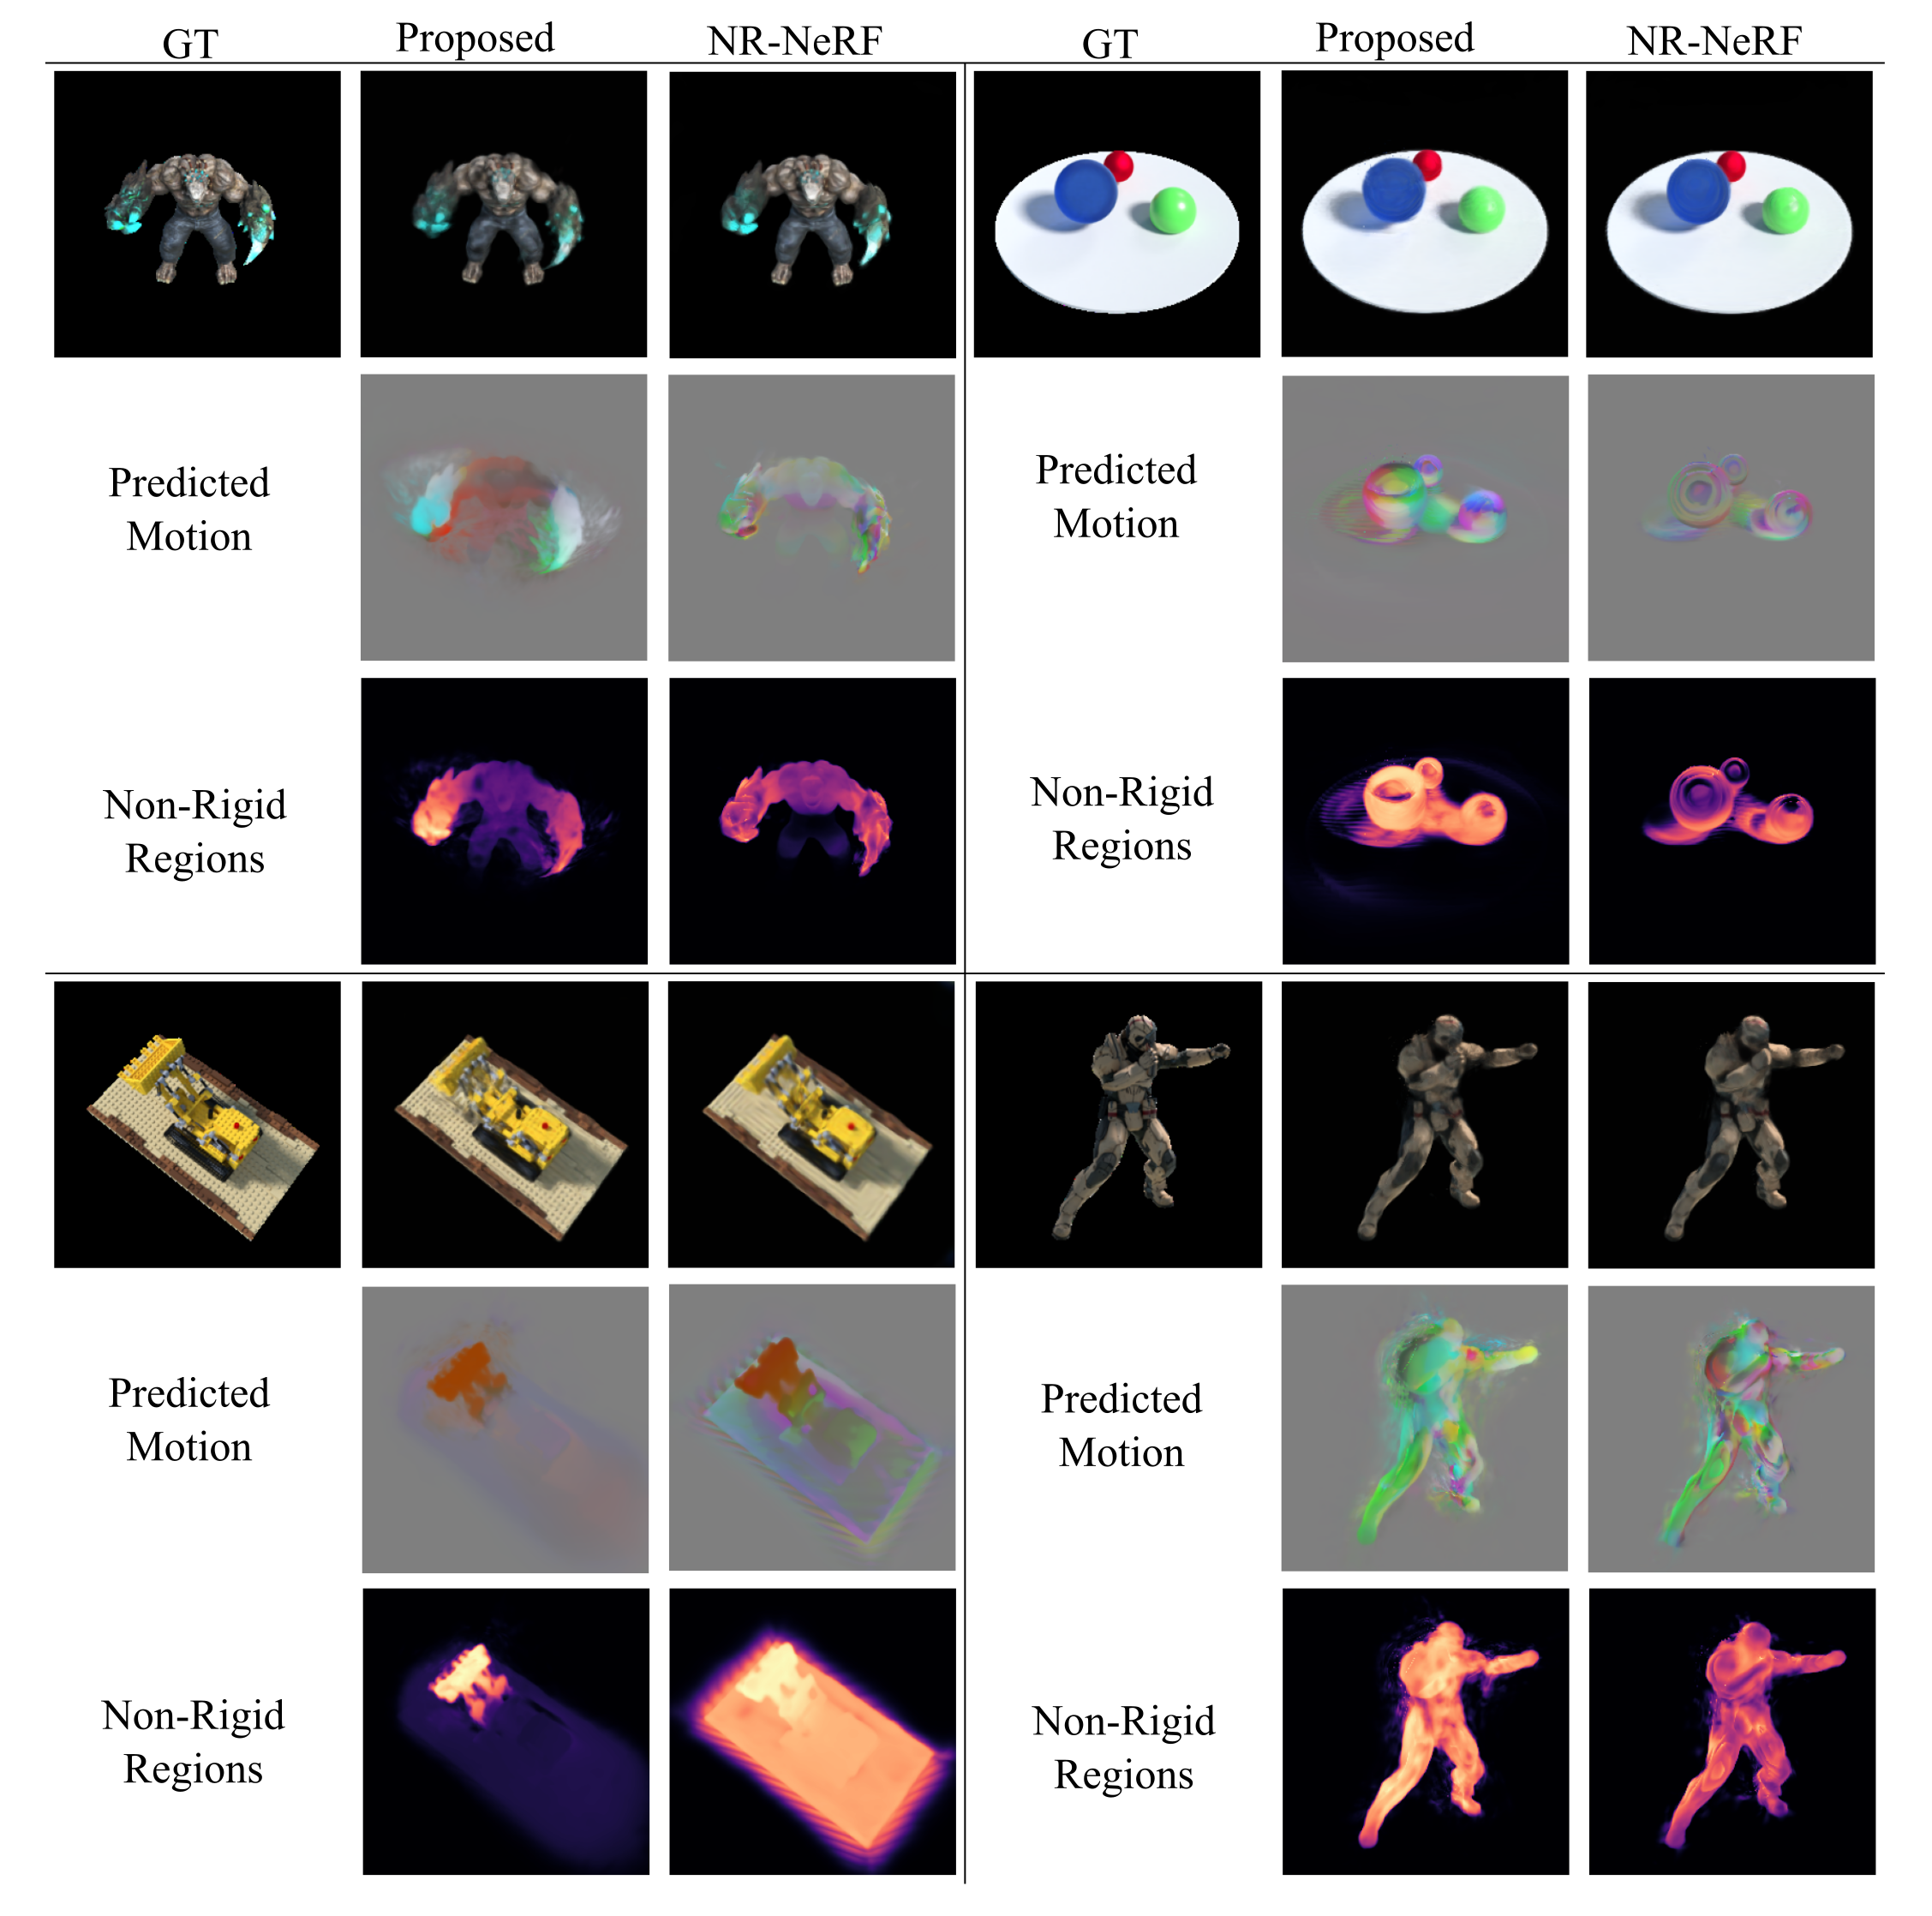
\includegraphics[width=\textwidth]{compare}
    \caption{
        \label{fig:qual_cmp}
        \textbf{Visual comparison of Spline-NeRF to NR-NeRF.}
        Results comparing movement in our implementation of NR-NeRF~\cite{tretschk2021nonrigid} versus the proposed approach for using Bezier splines for modelling movement. The direction of motion is shown by color, distance is shown by intensity, and gray is 0 motion. Non-rigid regions are characterized by higher intensity. There is substantial difference in the predicted motion, and this can be visually seen in the Mutant and Hook scenes (top left, bottom right respectively), where NR-NeRF predicts very noisy 3D flow, but our approach is coherent within spatial regions. There is also a large difference in rigidity, where the spline has higher coherence of non-rigid regions. This is especially noticeable in the Lego scene (bottom left), where NR-NeRF makes the entire model non-rigid, but adding a spline isolates the loader on the tractor to be non-rigid. We expect this is because splines will be coherent in similar regions, the rigidity is less needed to compensate for error, and the scale of movement in nearby points must be similar. For an MLP, it may predict different scales of motion for nearby points, but rigidity can compensate for this.
        \
        The quality of the output is similar. In some portions, NR-NeRF captures higher quality output, such as in the shadows of the balls, or in the crispness of the Mutant's blue claws. On the other hand, the spline more accurately captures the knobs and shadows of the knobs on the Lego scene.
    }
\end{figure*}

\begin{figure*}[!ht]
    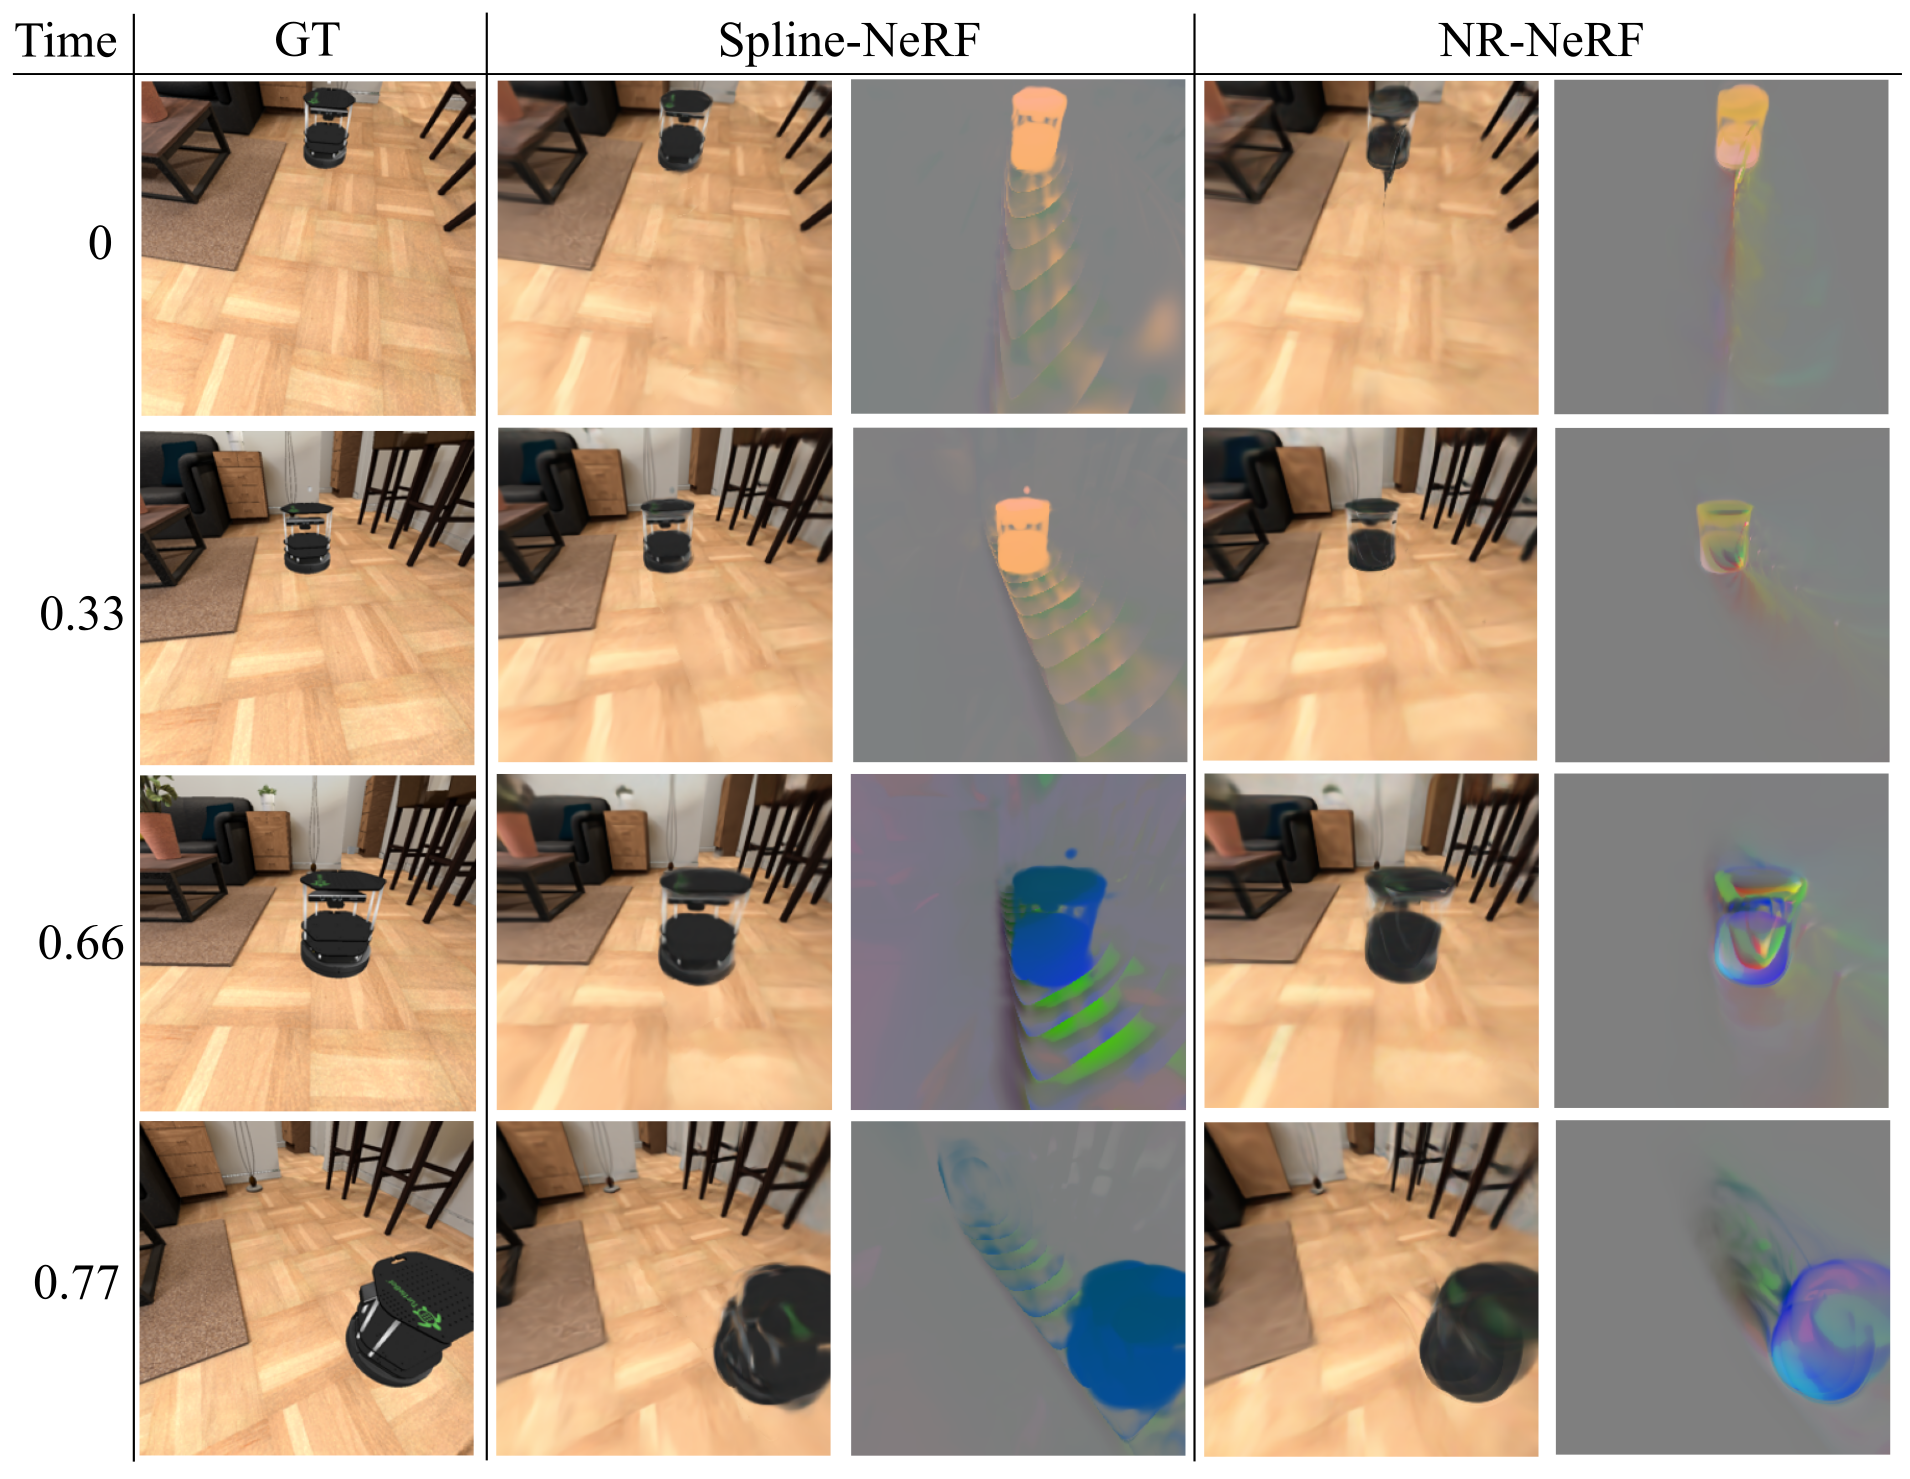
\includegraphics[width=\textwidth]{gibson_cmp}
    \caption{
        \label{fig:gib_cmp}
        \textbf{Visual comparison of Spline-NeRF to NR-NeRF on Gibson Dataset.} Our method produces coherent movement as compared to NR-NeRF, and is also visually more coherent, despite having a lower PSNR and MS-SSIM. It can be easily seen that the TurtleBot in NR-NeRF has artifacts, and does not move as a whole unit, whereas Spline-NeRF moves the whole robot uniformly. We do not include samples around $t=1$, since they are relatively sparse, and both our approach and NR-NeRF produce low-quality reconstructions.
    }
    \vspace{-6mm}
\end{figure*}
